%!TEX root = thesis.tex
\chapter{Results}


Results could be achieved for the building energy analysis, the PV analysis and the combined analysis, as described in this chapter.

\section{Building Energy Analysis}
	
	The optimal configurations of the ASF can be visualised using carpet-plots. For a classical building analysis this was done for every hour of the year. Figures \ref{f:DIVAx} and \ref{f:DIVAy} show the optimizing altitude and azimuth angles for heating, cooling, lighting and total building energy demand, respectively. Carpet plots detailing the optimal altitude angles to minimise the (a) heating demand, (b) cooling demand, (c) lighting demand, and (d) total building energy demand. In figure arker colors represent closed positions, whereas brighter colors correspond to open positions. To optimize heating and lighting, open positions (corresponding to large altitude angles) are favorable, cooling is optimized by using closed positions (corresponding to small altitude angles). The overall optimized solutions follow the corresponding patterns at the hours of importance.  

	\begin{figure*}
		\begin{center}
		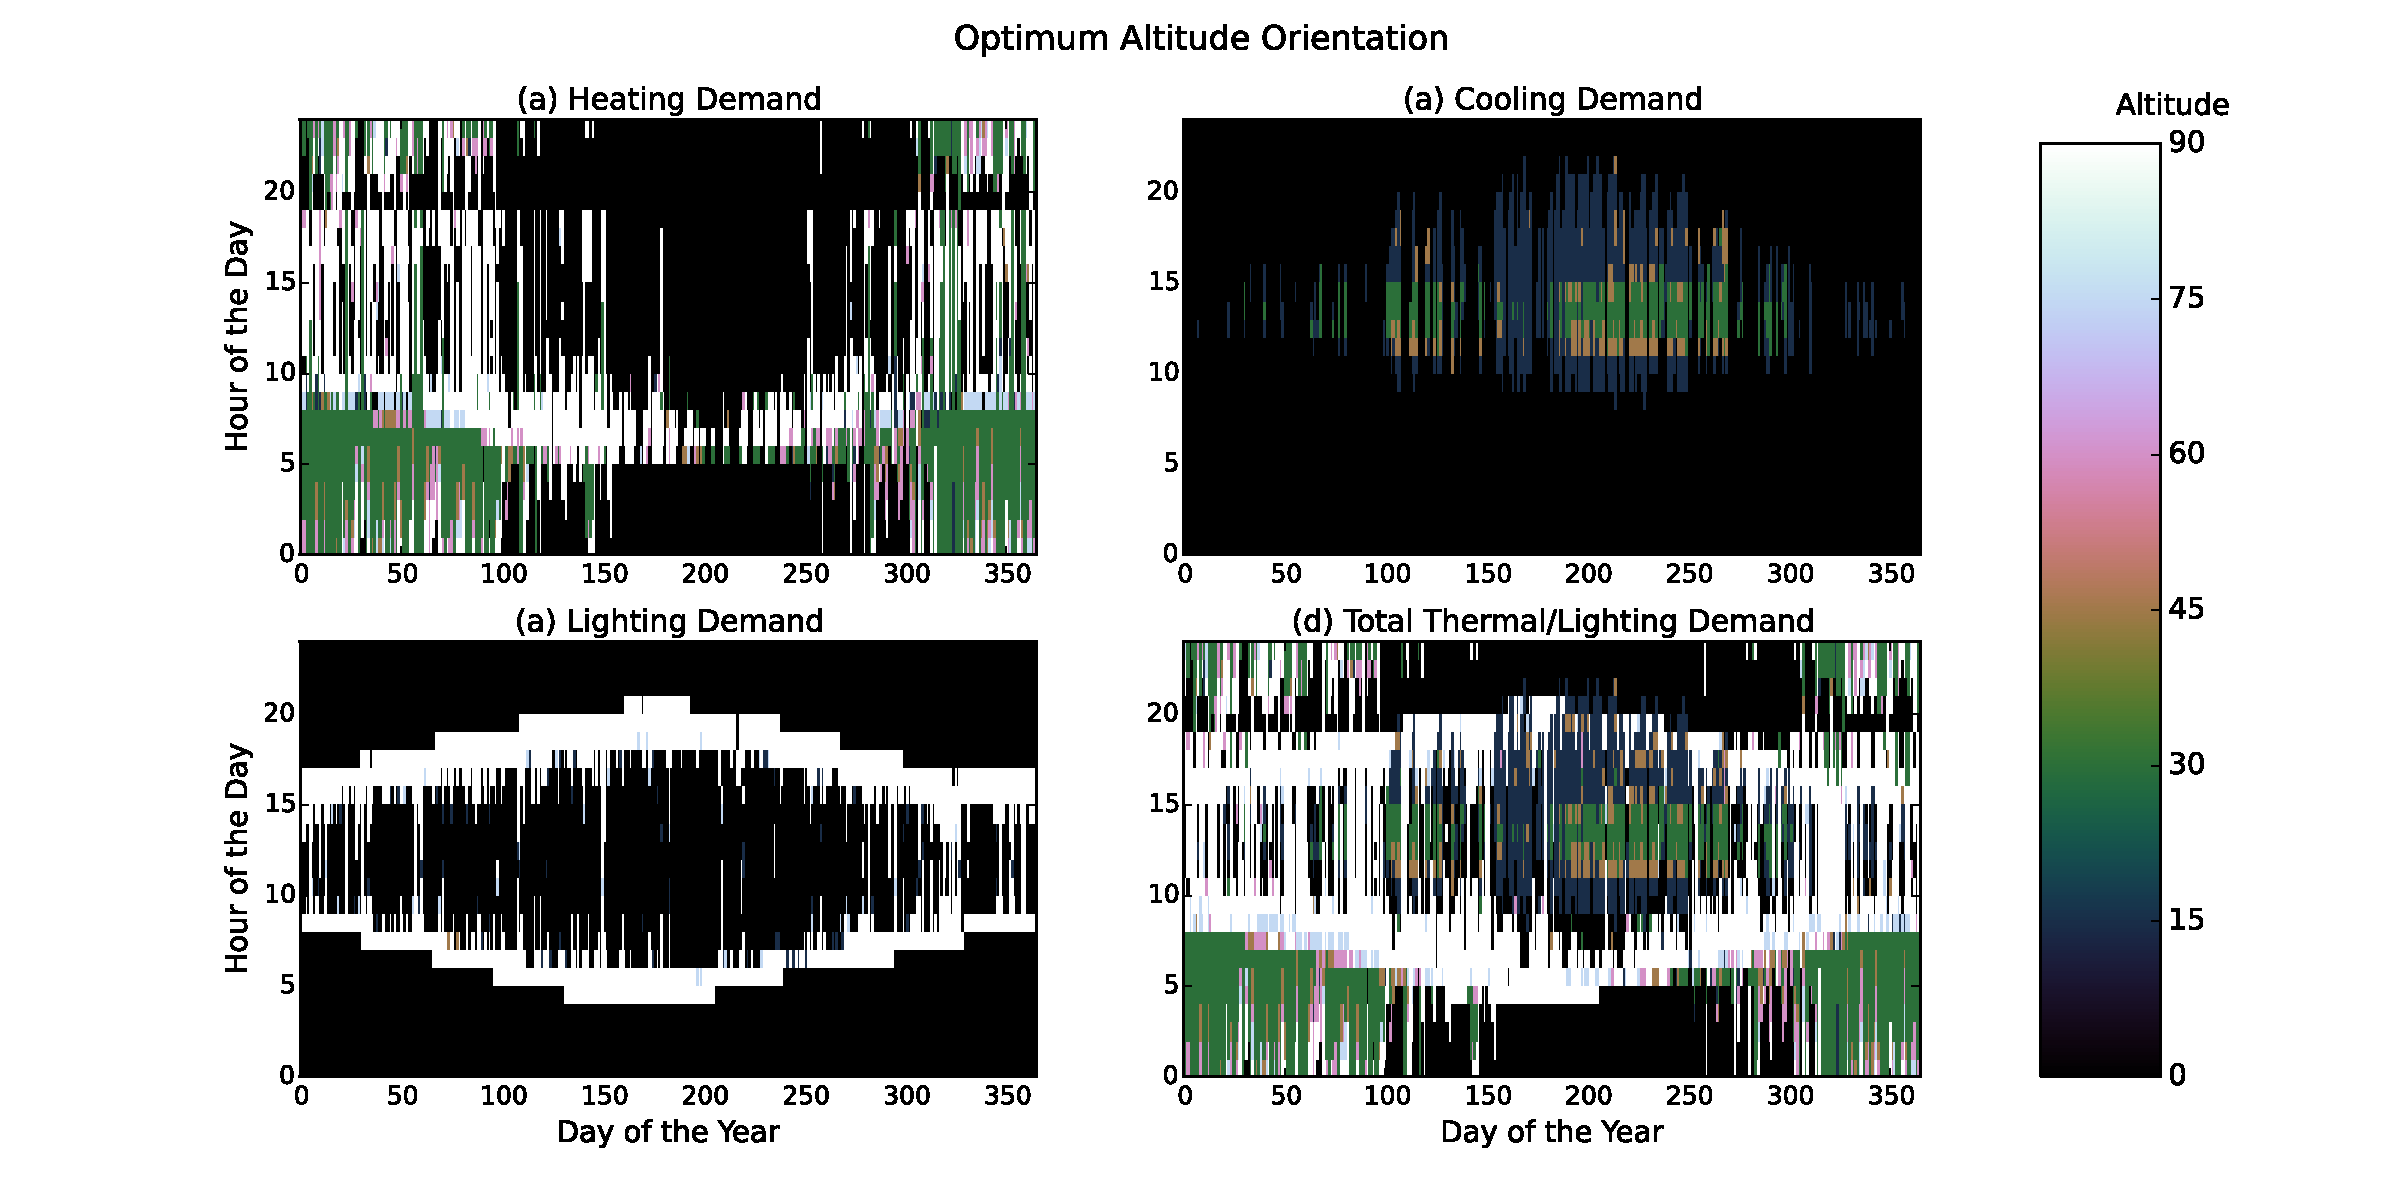
\includegraphics[width=\textwidth, trim= 0cm 0cm 0cm 0cm,clip]{DIVAx}
		\caption{Carpet plots detailing the optimal altitude angles to minimise the (a) heating demand, (b) cooling demand, (c) lighting demand, and (d) total building energy demand. Darker colors represent closed positions, whereas brighter colors correspond to open positions. To optimize heating and lighting, open positions are favorable, cooling is optimized by using closed positions.}
		\label{f:DIVAx}
		\end{center}
	\end{figure*}


	\begin{figure*}
		\begin{center}
		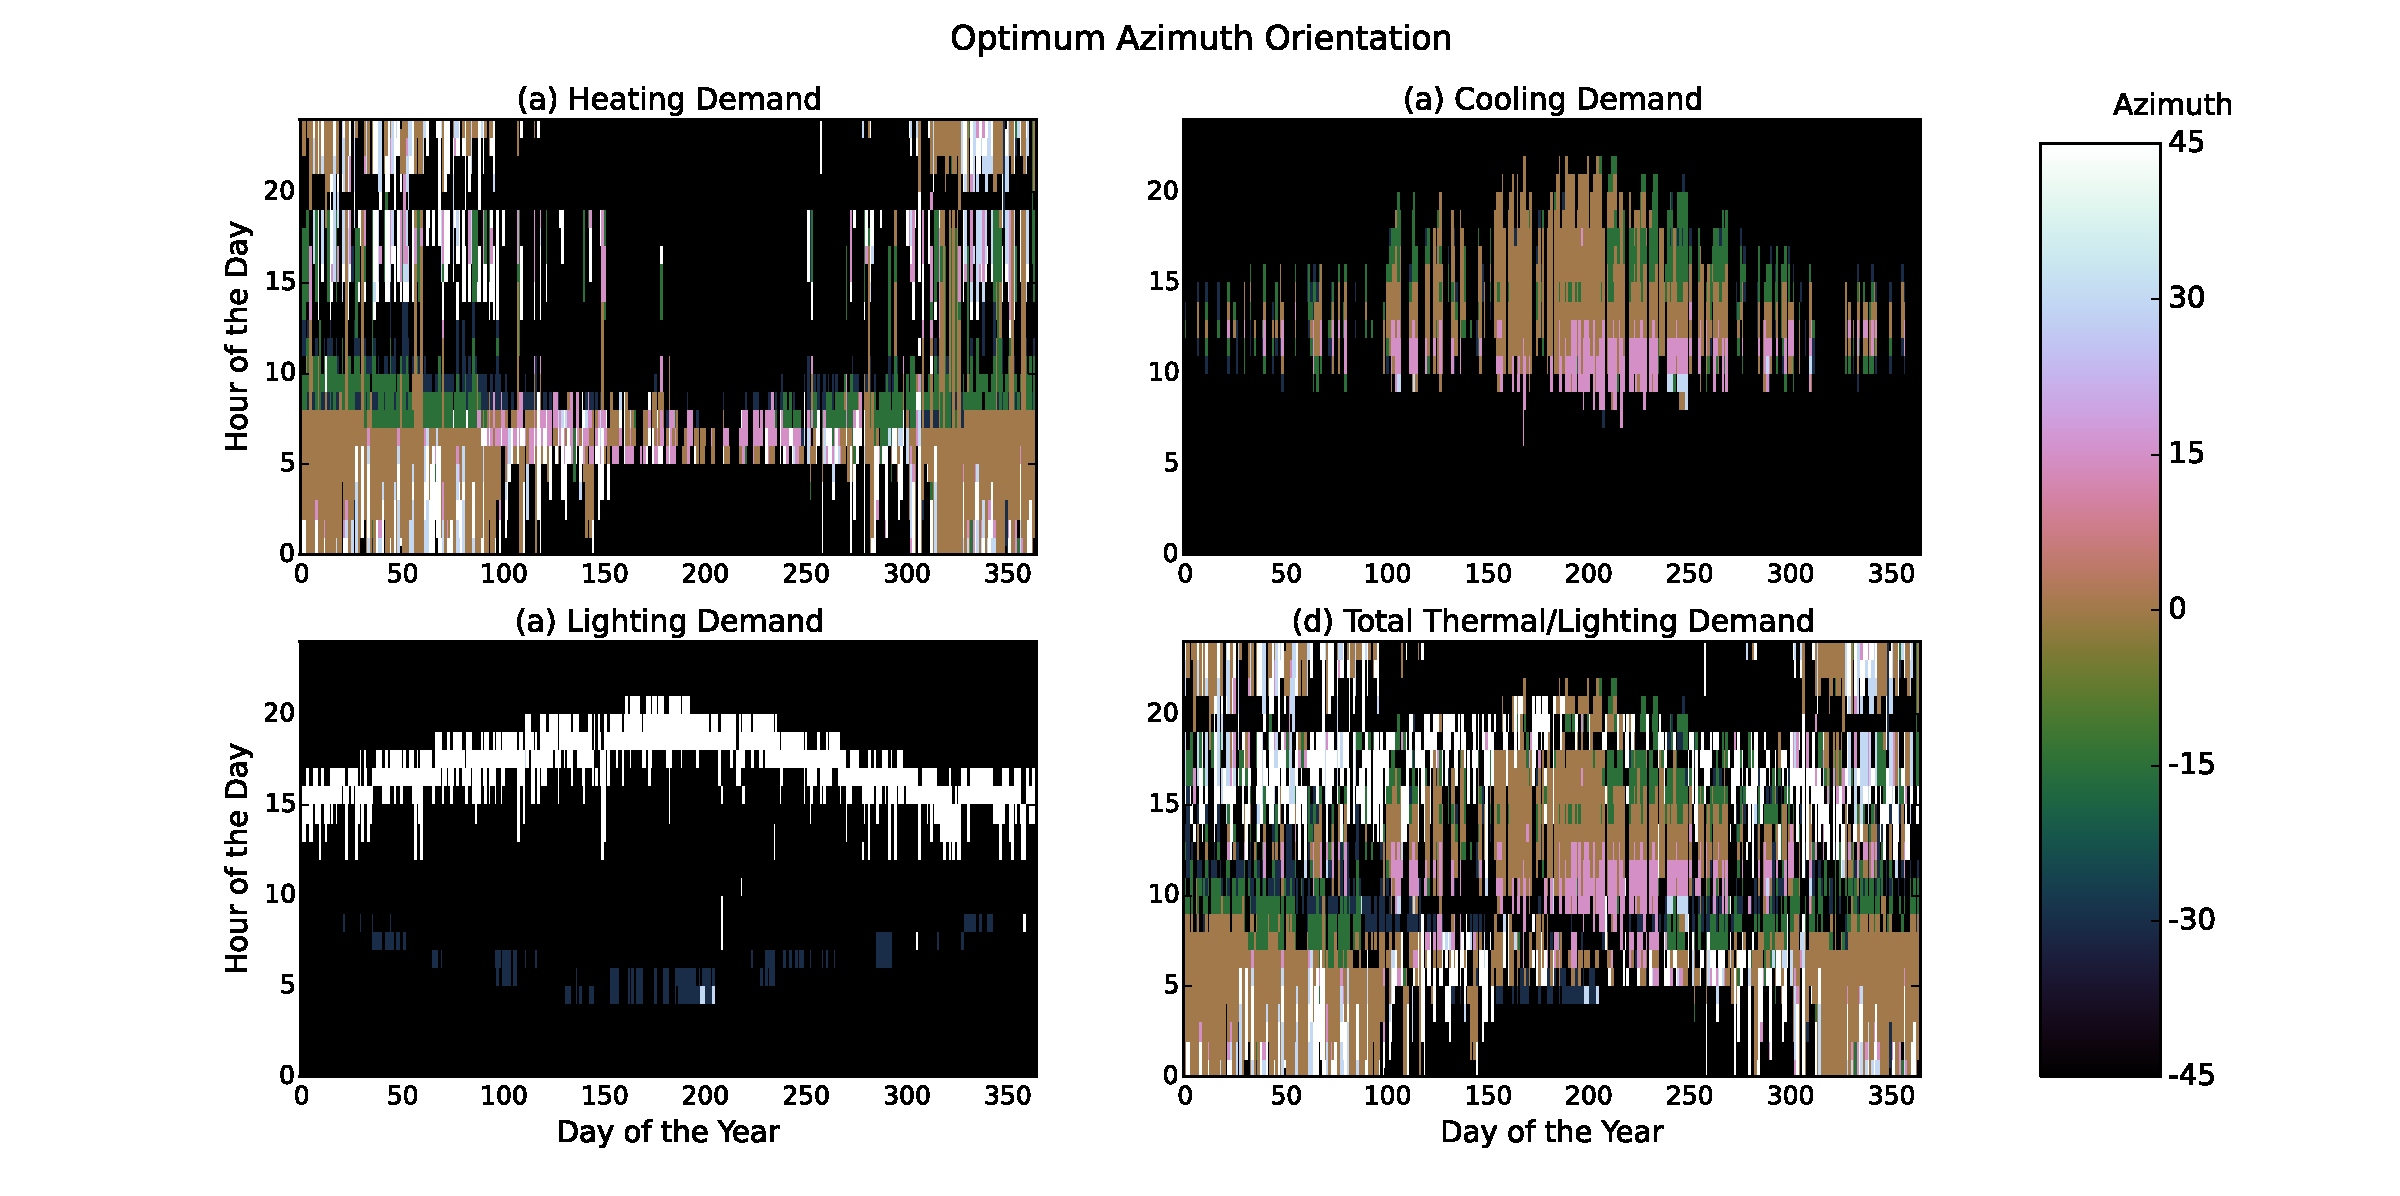
\includegraphics[width=\textwidth, trim= 0cm 0cm 0cm 0cm,clip]{DIVAy}
		\caption{Carpet plots detailing the optimal azimuth angles to minimise the (a) heating demand, (b) cooling demand, (c) lighting demand, and (d) total building energy demand. Cooling is minimized by bocking the sun, wheras lighting and heating is minimized by opening the facade to let the insolation in.}
		\label{f:DIVAy}
		\end{center}
	\end{figure*}


	\begin{figure*}
		\begin{center}
		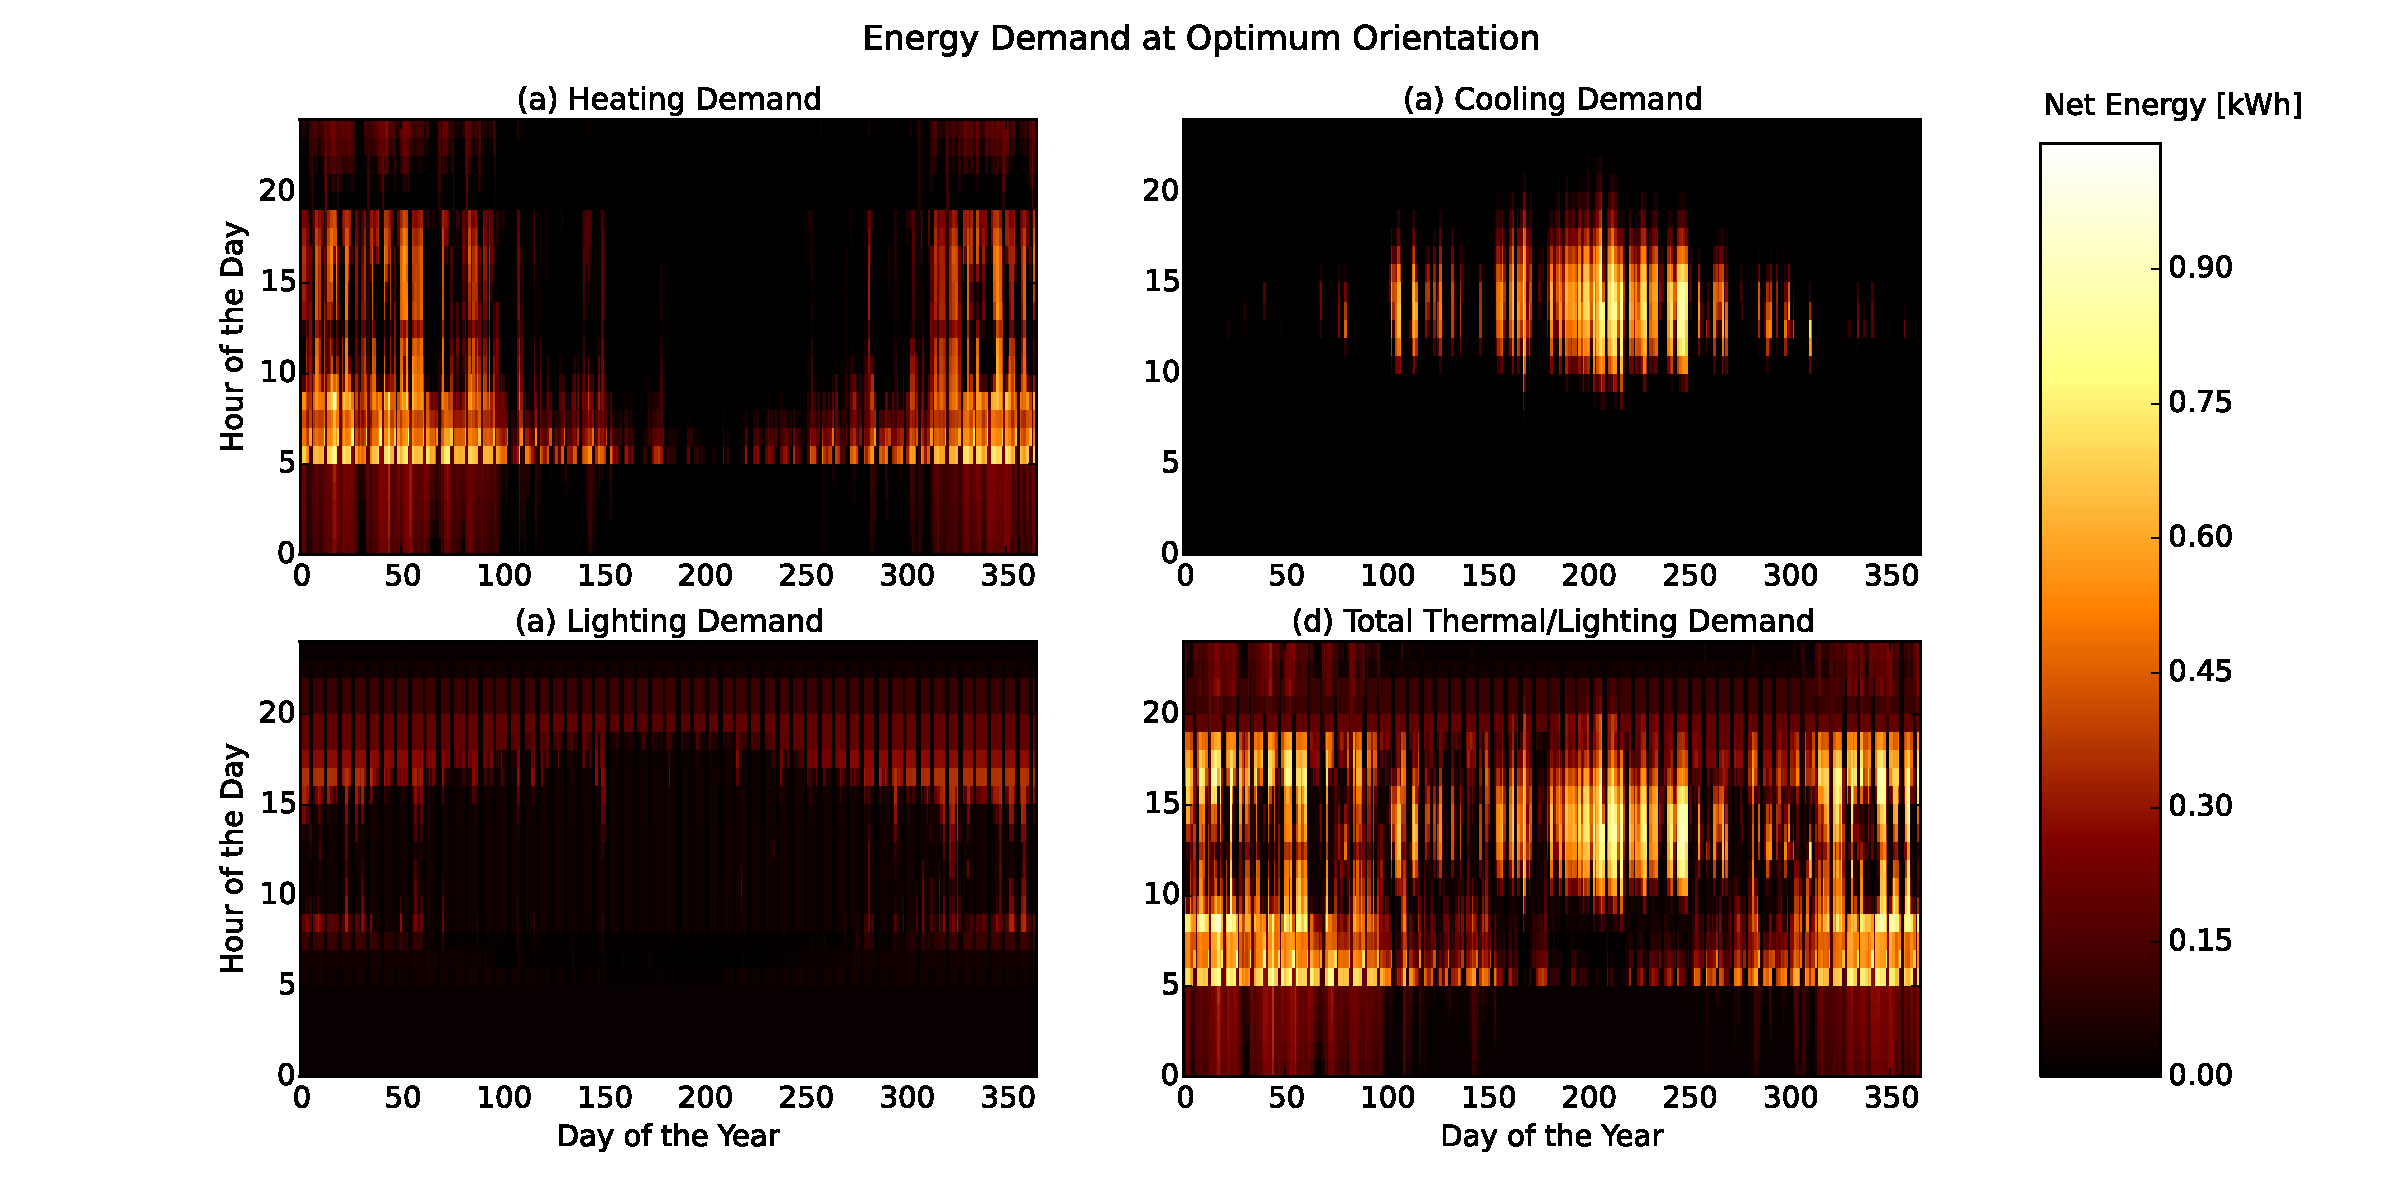
\includegraphics[width=\textwidth, trim= 0cm 0cm 0cm 0cm,clip]{DIVAe}
		\caption{Carpet plots detailing the net energy consumption. Each square represents the total energy consumption for that specific hour of the entire month. Red colours detail the energy demand, while blue colours detail the energy supply.}
		\label{f:DIVAe}
		\end{center}
	\end{figure*}
	
\section{Radiation and PV Analysis}
	
	The detailed radiation pattern on the PV panels was analised and a detailed estimation of the PV electricity production was performed. 
	

	\subsection{Grid Convergence}

		With a larger gridsize, results are less accurate. In order to study this effect, a grid convergence study was conducted. Figure \ref{f:gridConvergence} shows the grid size dependency of the total radiation on the asf. It can be seen that a smaller gridsize leads to larger deviations. The normalization is done by dividing the total radiation of each gridsize by the total radiation with gridsize 12.5\,mm. While for a gridsize of 400\,mm the average deviation is over 10\%, the deviation goes down to below 1\% for a grid size of 25\,mm. 25\,mm was therefore taken as the gridsize of all simulations, as it gives accurate results, while still being computationaly feasible. 

		\begin{figure*}
			\begin{center}
			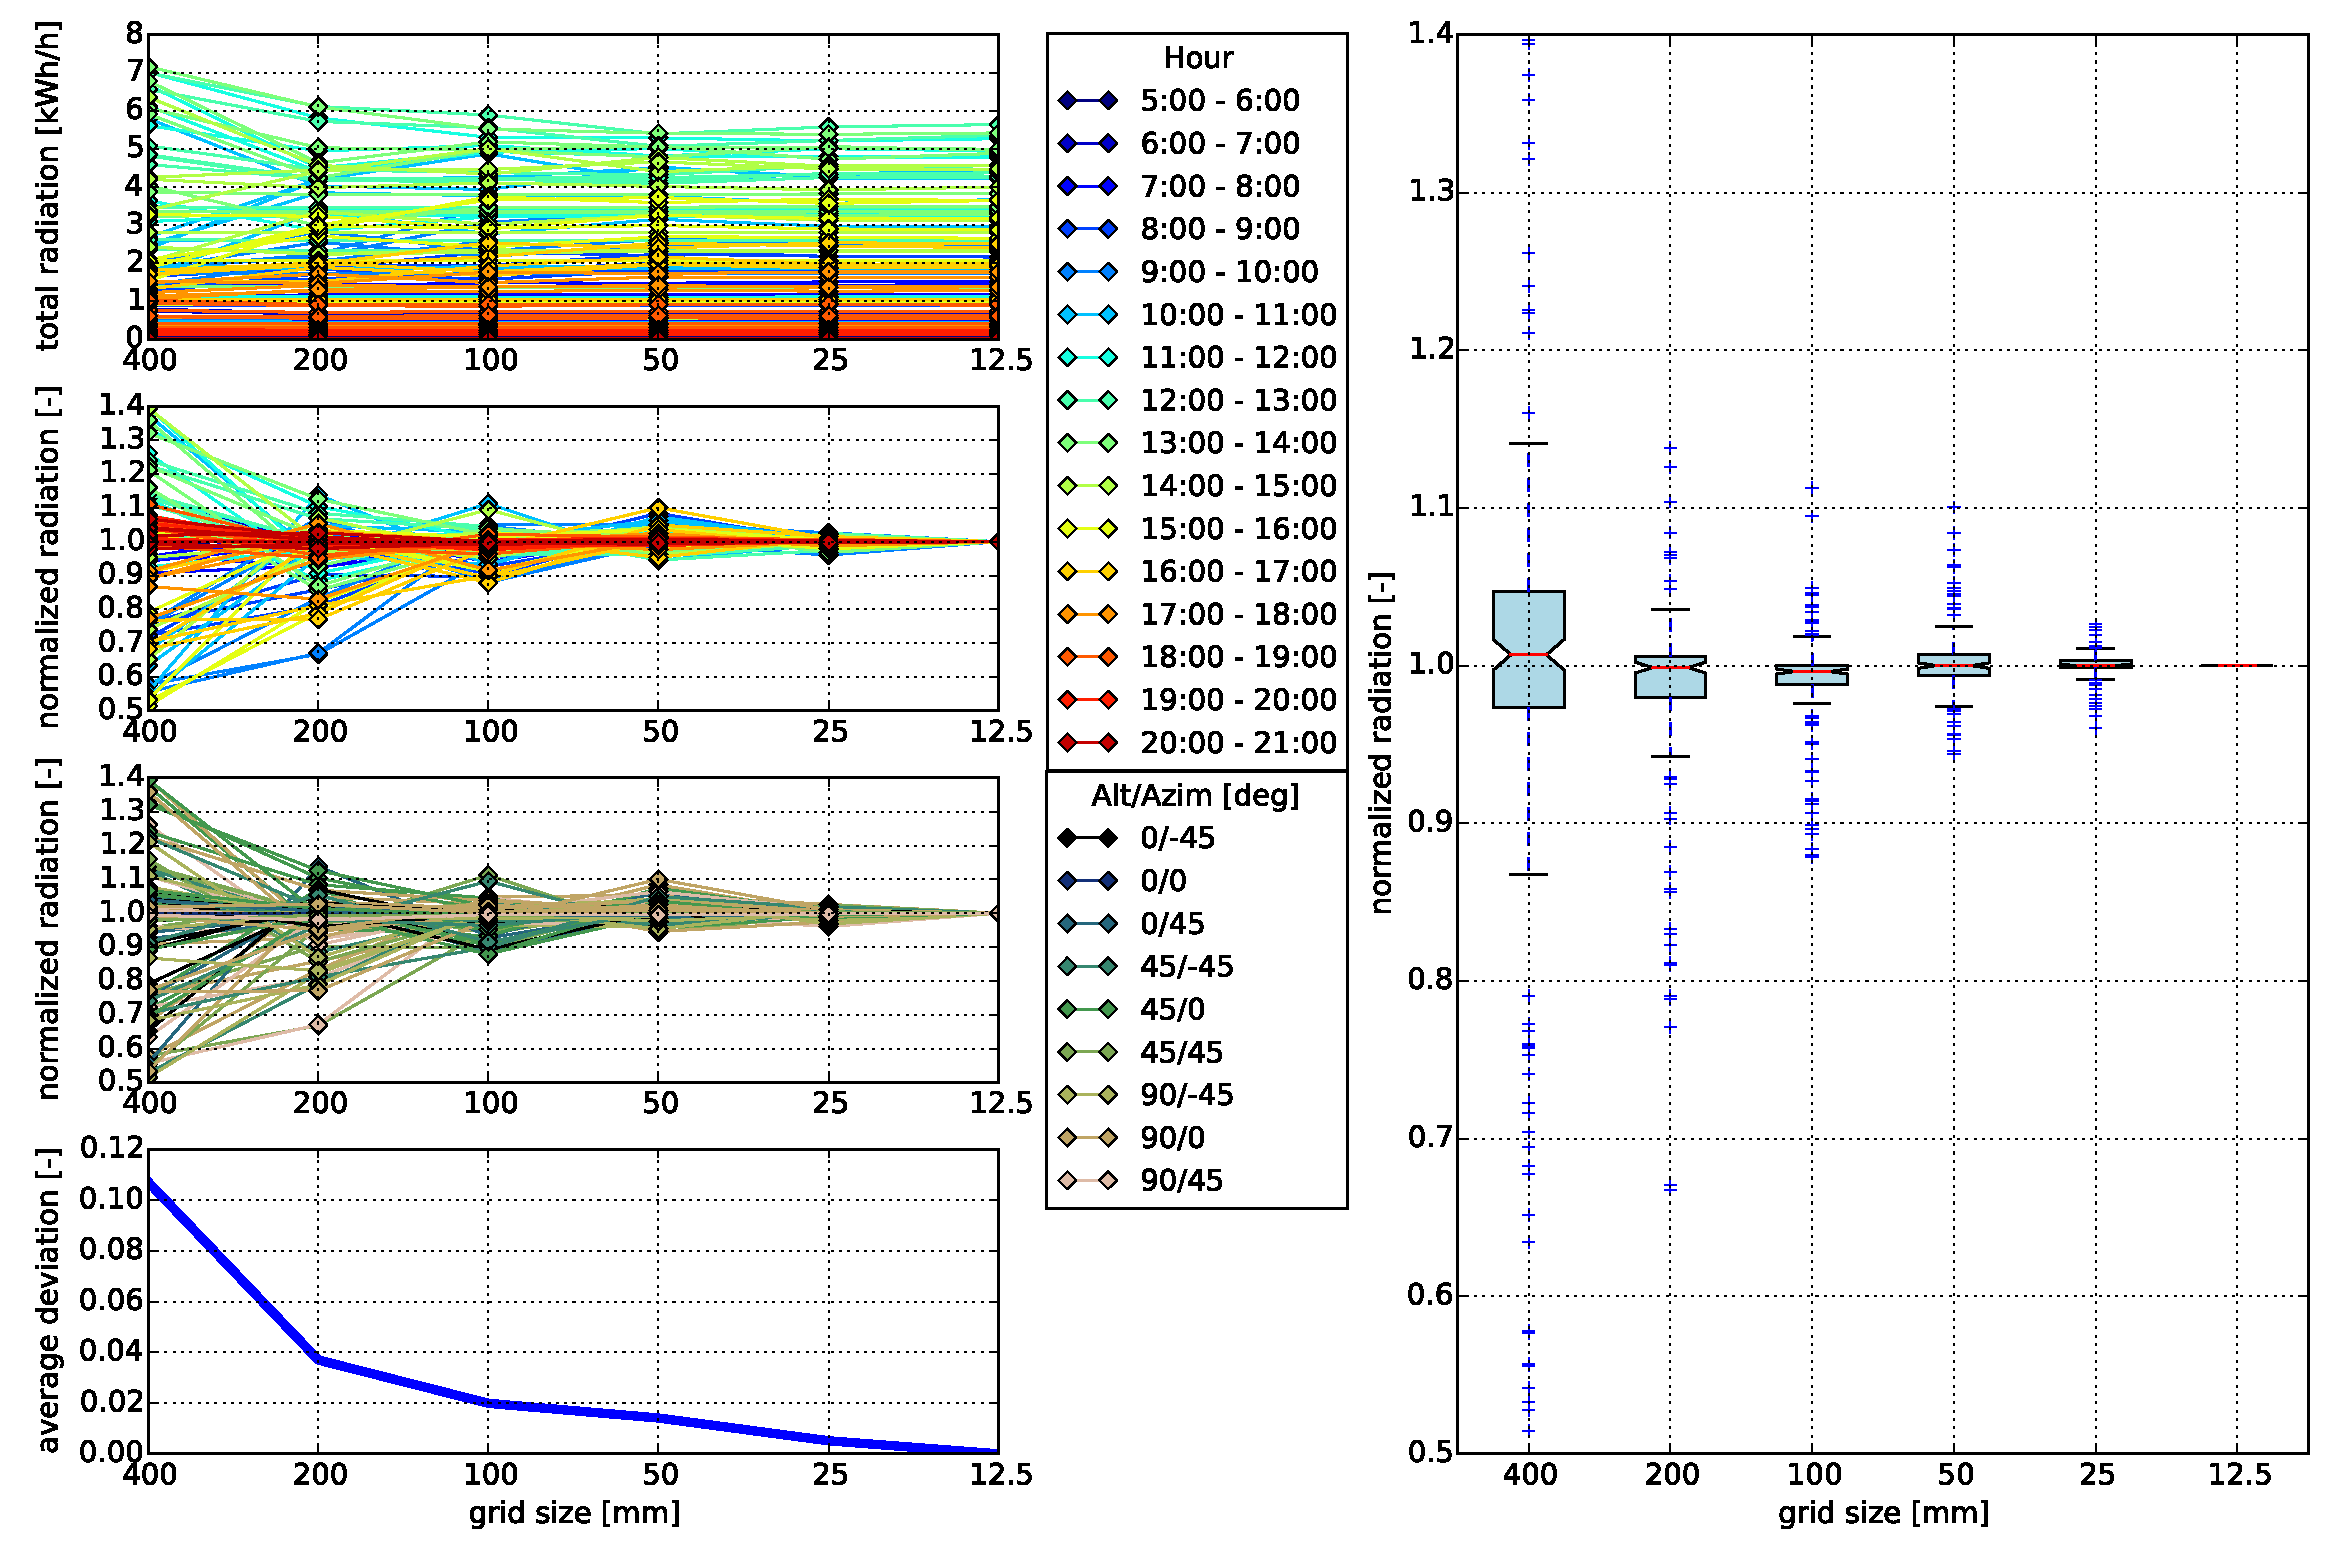
\includegraphics[width=\textwidth, trim= 0cm 0cm 0cm 0cm,clip]{gridConvergence.pdf}
			\caption{Grid convergence evaluation}
			\label{f:gridConvergence}
			\end{center}
		\end{figure*}

	\subsection{Comparison of Sun Tracking to Optimized Solution}

		In order to evaluate the optimum configuration for PV production, simulations using sun-tracking were compared to simulations evaluating the basecase of 49 different combinations (i.e. 7 different azimuth and altitude angles). In figure \ref{f:compareSuntracking} it can be seen that while the radiation on the panels is pretty similar for both sun tracking and the optimized solution, the PV electricity production of the optimized solution is significantly higher than the sun-tracking solution in the afternoon hours. This is caused by the layout of the PV panels, longitudinal shading causes high power losses \cite{hofer2015PVSEC}, thus the optimized solution decreases the longitudinal shading compared to sun-tracking. 

		\begin{figure*}
			\begin{center}
			\includegraphics[width=\textwidth, trim= 0cm 0cm 0cm 0cm,clip]{compareSuntracking}
			\caption{Comparison of optimized solution to sun-tracking. a) average radiation on panels compared to radiation without shading b) PV electricity production comparison c) efficiency comparison}
			\label{f:compareSuntracking}
			\end{center}
		\end{figure*}




\section{Combined Evaluation}

	By combining results for building energy simulations and PV electricity production, the overall optimum configurations can be found. Figure \ref{fig:carpetplot} details carpet-plots of the facade optimised to maximise PV generation, and minimise heating, cooling and lighting demands independently. It can be see that open configurations (light coloured) are chosen to minimise the building heating demands during the winter months and early mornings of spring and autumn. Likewise closed configurations (dark colours) are the preferred solutions to minimise the cooling demand during the summer months. Lighting control is only apparent during the twilight hours where the facade prefers an open position to avoid the use of artificial lighting. The PV optimisation follows a solar tracking model for most hours and as far as the limited range of angles allows. This causes some issues during twilight summer hours as the actuator cannot physically align itself normal to the sunlight. 




	\begin{figure*}
	\begin{center}
	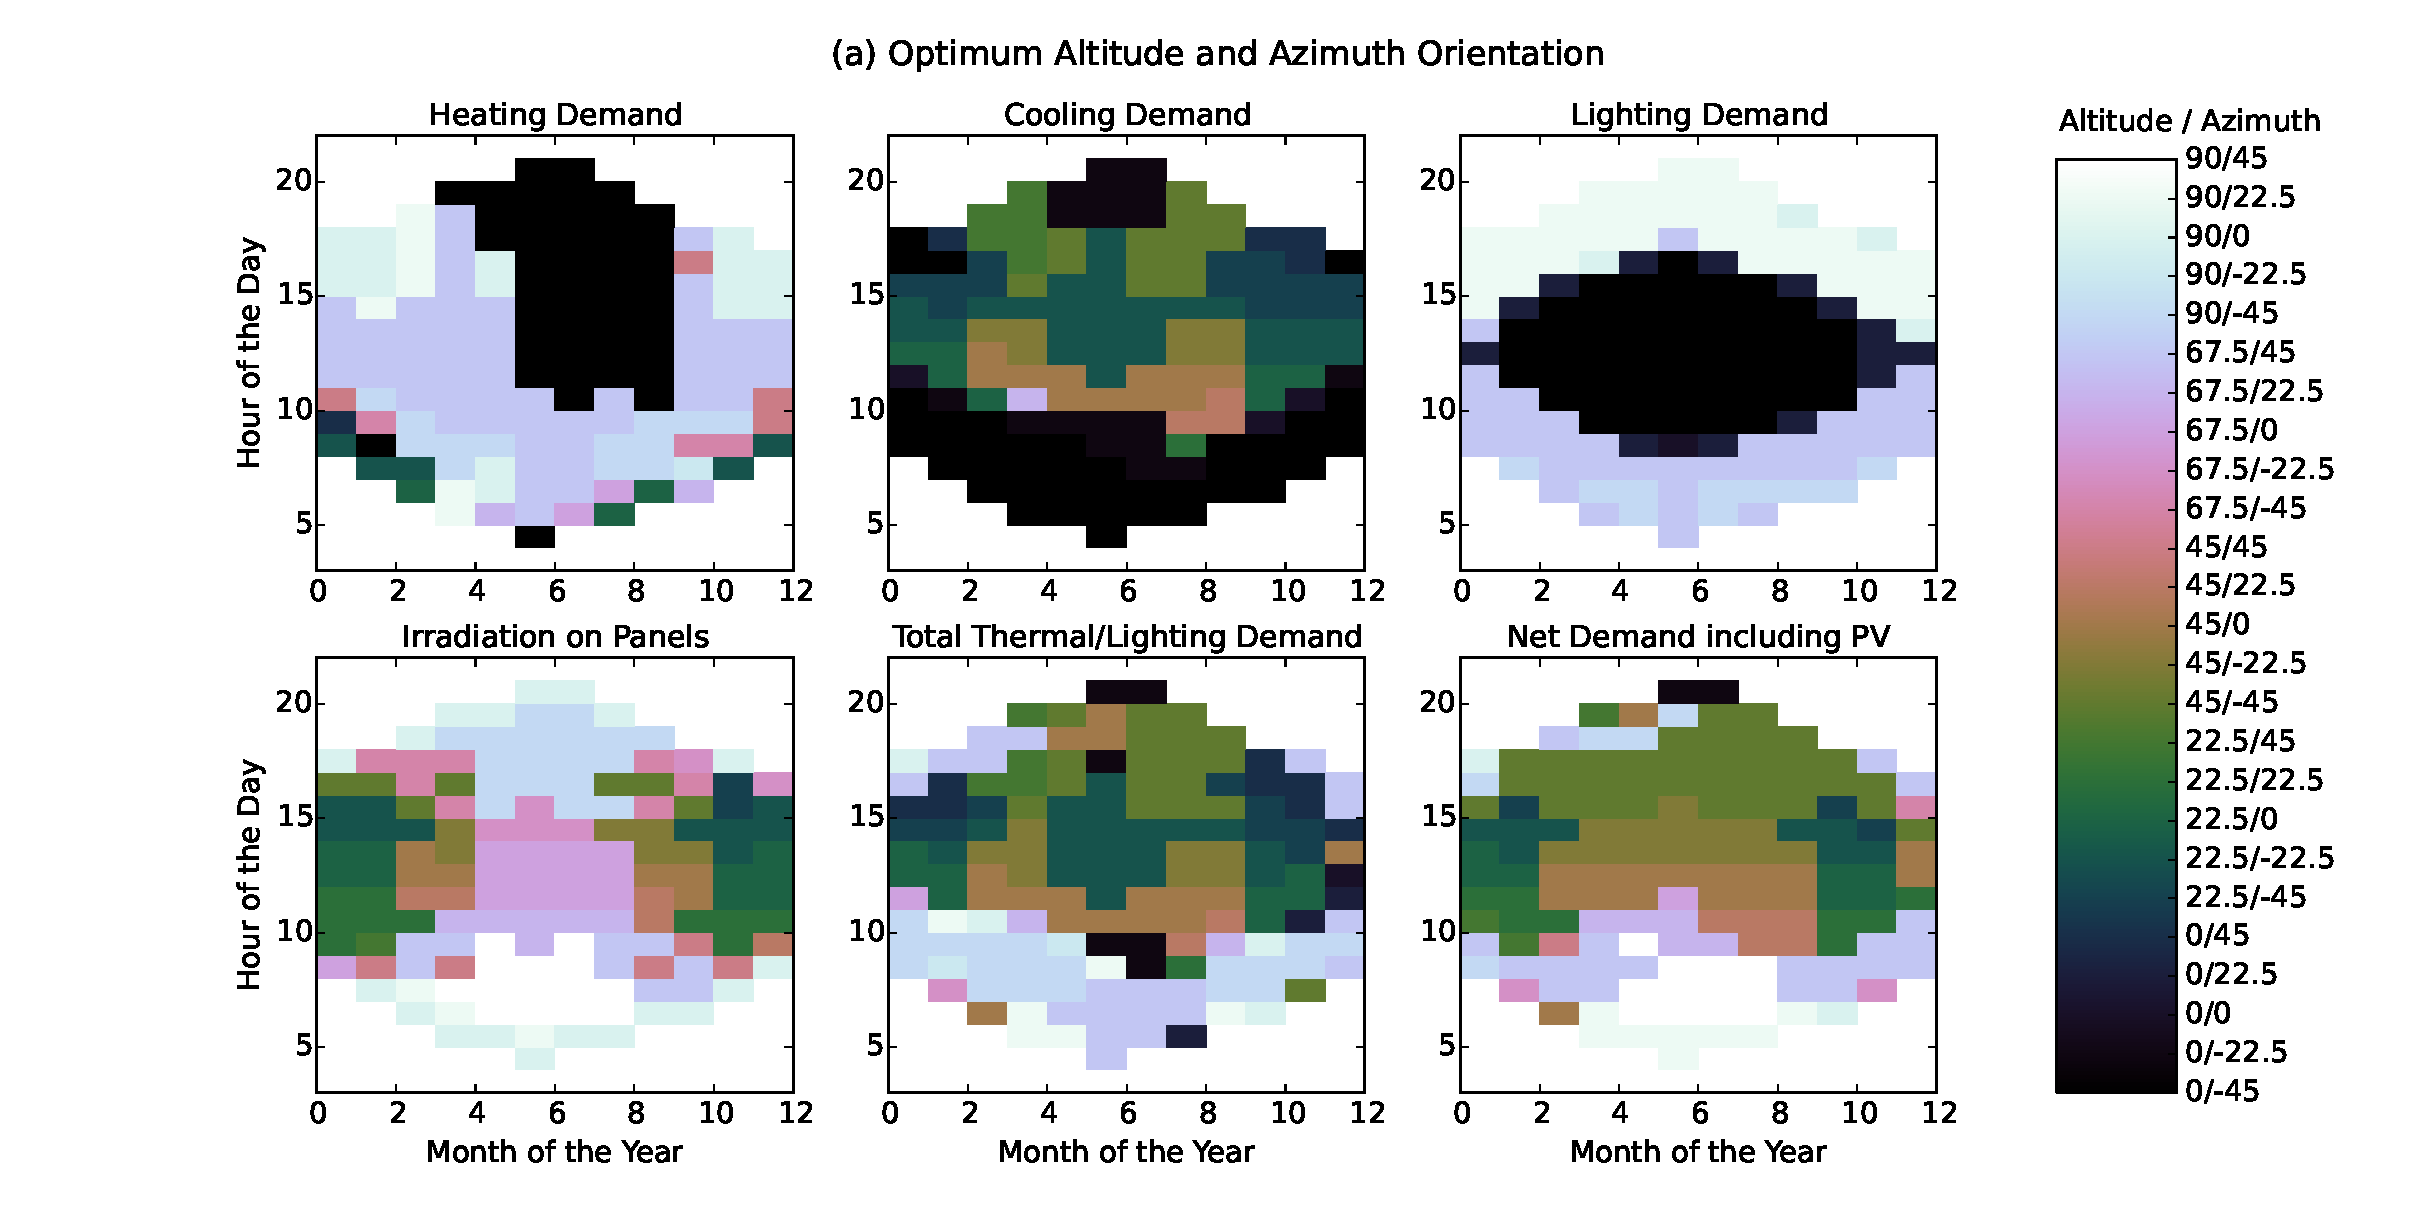
\includegraphics[width=\textwidth, trim= 0cm 0cm 0cm 0cm,clip]{carpetplot_angles.eps}
	\caption{Carpet plots detailing the optimal configuration to minimise the (a) heating demand, (b) cooling demand, (c) lighting demand, and (d) maximise irradiance on PV panels. Each configuration is represented by an angle of orientation around the x-axis (Altitude) and y-axis (Azimuth) as seen in the legend. Figure (e) details the combinations for optimum building thermal management without PV production. (f) also includes the PV production}
	\label{fig:carpetplot}
	\end{center}
	\end{figure*}

	\begin{figure*}
	\begin{center}
	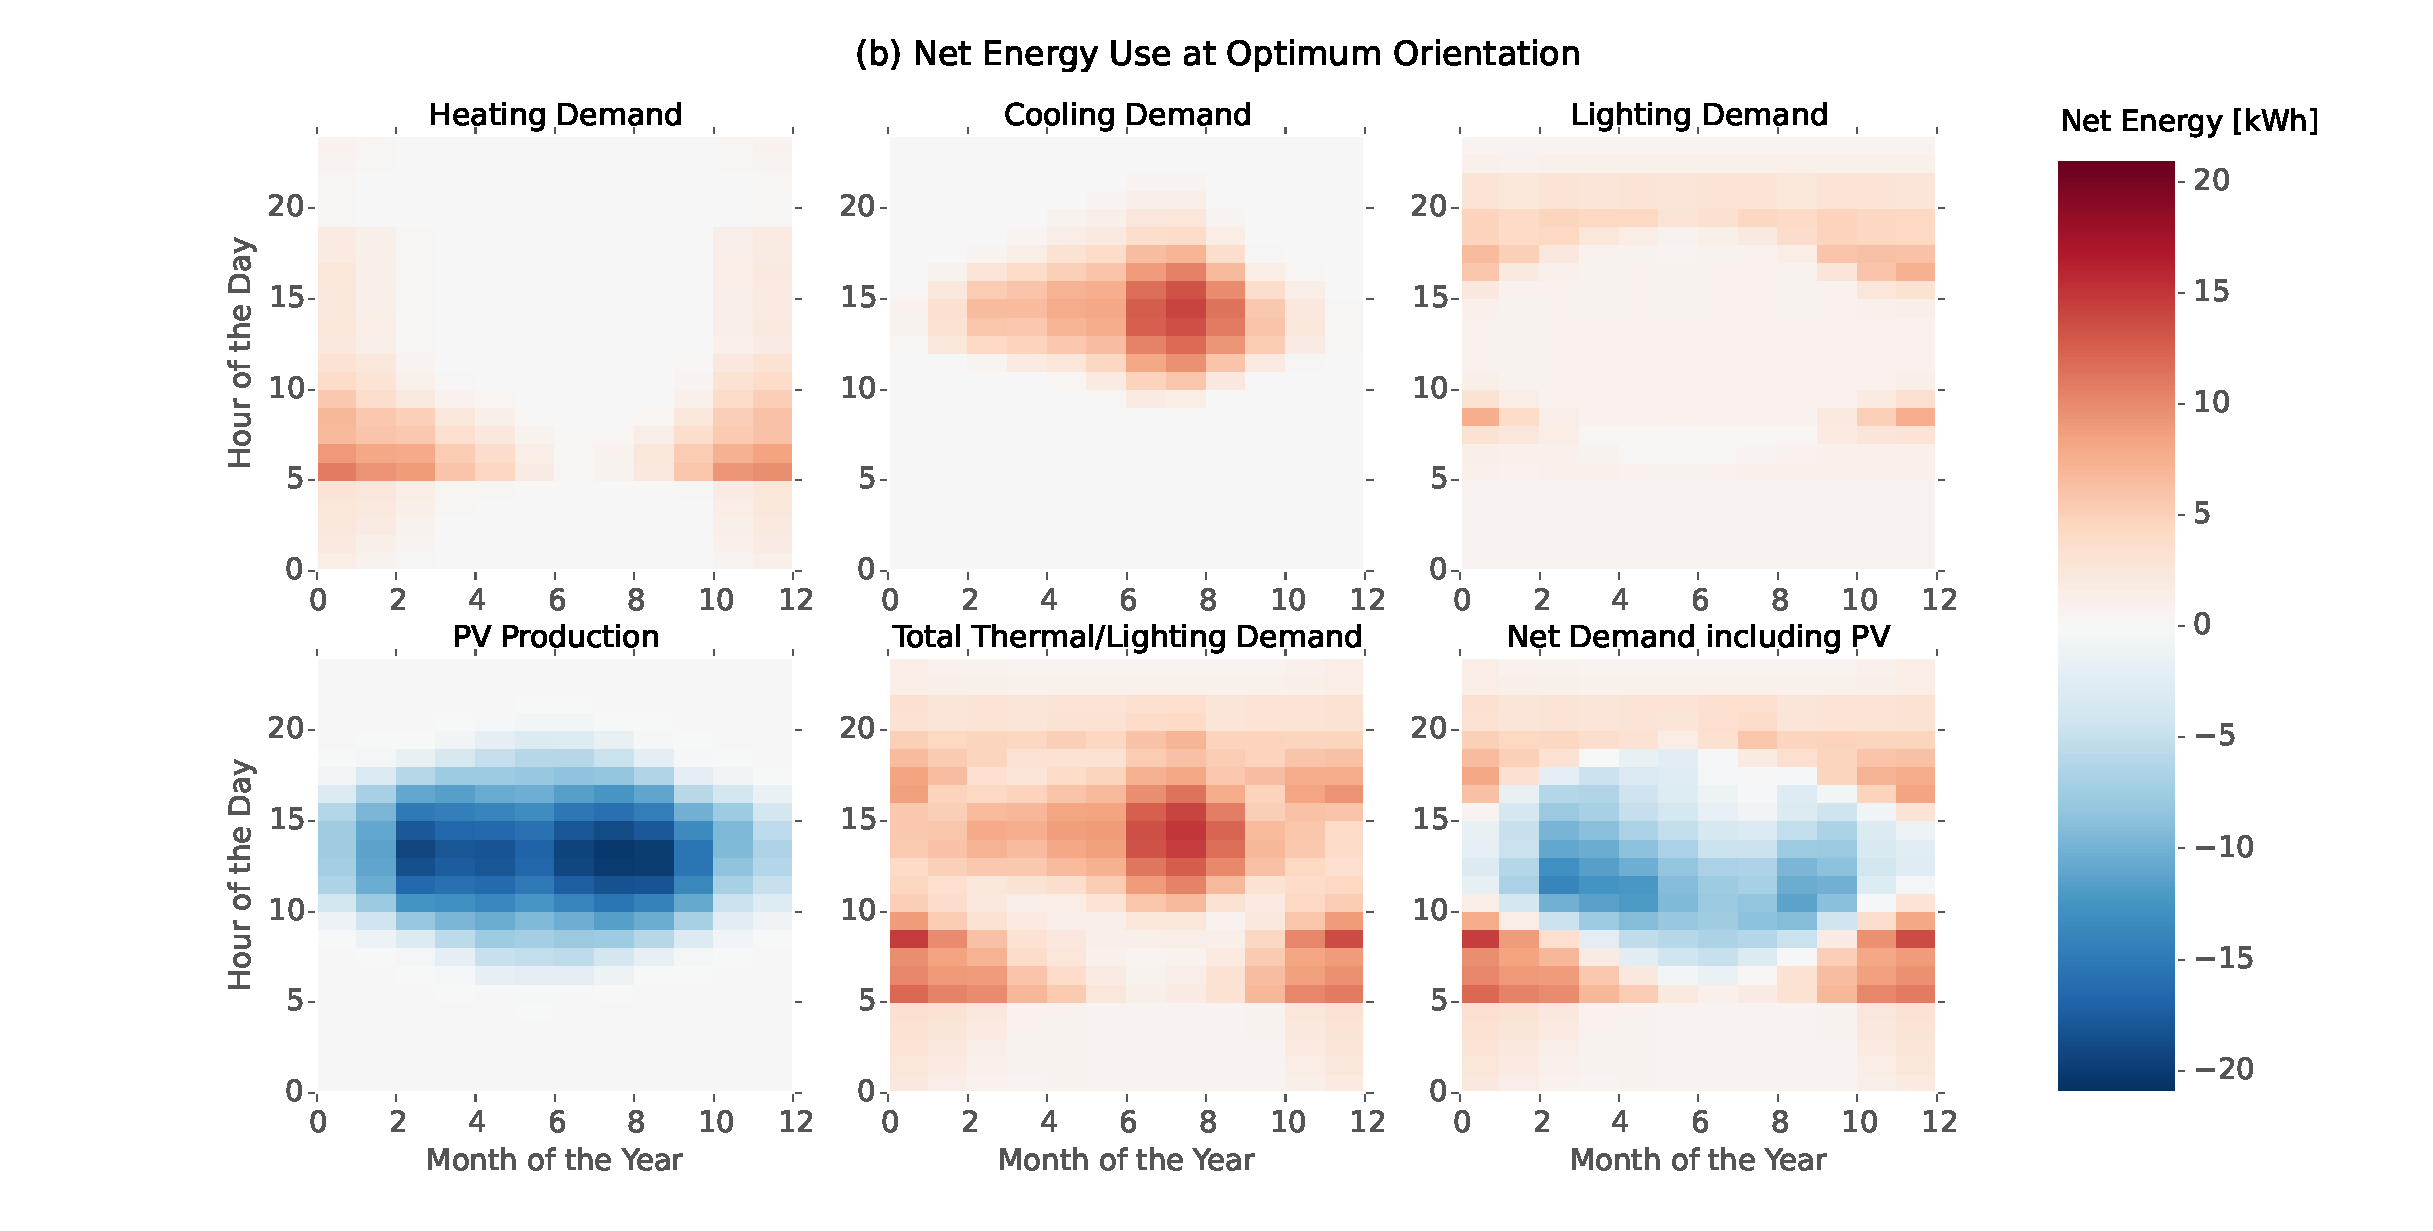
\includegraphics[width=\textwidth, trim= 0cm 0cm 0cm 0cm,clip]{carpetplot_energy.eps}
	\caption{Carpet plots detailing the net energy consumption. Each square represents the total energy consumption for that specific hour of the entire month. Red colours detail the energy demand, while blue colours detail the energy supply.}
	\label{fig:carpetplot_energy}
	\end{center}
	\end{figure*}



	When the four optimisation cases are combined to achieve the configurations for total energy minimisation we get some interesting results. There is a conflict in the summer evenings between minimising lighting and cooling demands. Likewise, we also see a conflict between heating and PV production during the winter months. The overall energy optimization including PV electricity production shows a strong tendency to follow the optimal PV production pattern. This, however changes if the building system becomes more inefficient. Less efficient heating for example, would result in configurations optimised for heating overpowering those of PV electricity generation.


	Figure \ref{fig:carpetplot_energy} shows the net energy use at these optimum angles. It is interesting to see how the combination of electricity generation and adaptive shading can compensate for the entire energy use during sunlit hours.

